% This file was created by matlab2tikz.
%
%The latest updates can be retrieved from
%  http://www.mathworks.com/matlabcentral/fileexchange/22022-matlab2tikz-matlab2tikz
%where you can also make suggestions and rate matlab2tikz.
%
\definecolor{mycolor1}{rgb}{0.85000,0.32500,0.09800}%
\definecolor{mycolor2}{rgb}{0.00000,0.44706,0.74118}%
\definecolor{mycolor3}{rgb}{0.92900,0.69400,0.12500}%
\definecolor{mycolor4}{rgb}{0.49400,0.18400,0.55600}%
\definecolor{mycolor5}{rgb}{0.85098,0.32549,0.09804}%
\definecolor{mycolor6}{rgb}{0.46600,0.67400,0.18800}%
\definecolor{mycolor7}{rgb}{0.30100,0.74500,0.93300}%
\definecolor{mycolor8}{rgb}{0.92941,0.69412,0.12549}%
\definecolor{mycolor9}{rgb}{0.63500,0.07800,0.18400}%
\definecolor{mycolor10}{rgb}{0.00000,0.44700,0.74100}%
\definecolor{mycolor11}{rgb}{0.49412,0.18431,0.55686}%
\definecolor{mycolor12}{rgb}{0.46667,0.67451,0.18824}%
\definecolor{mycolor13}{rgb}{0.50196,0.50196,0.50196}%
%
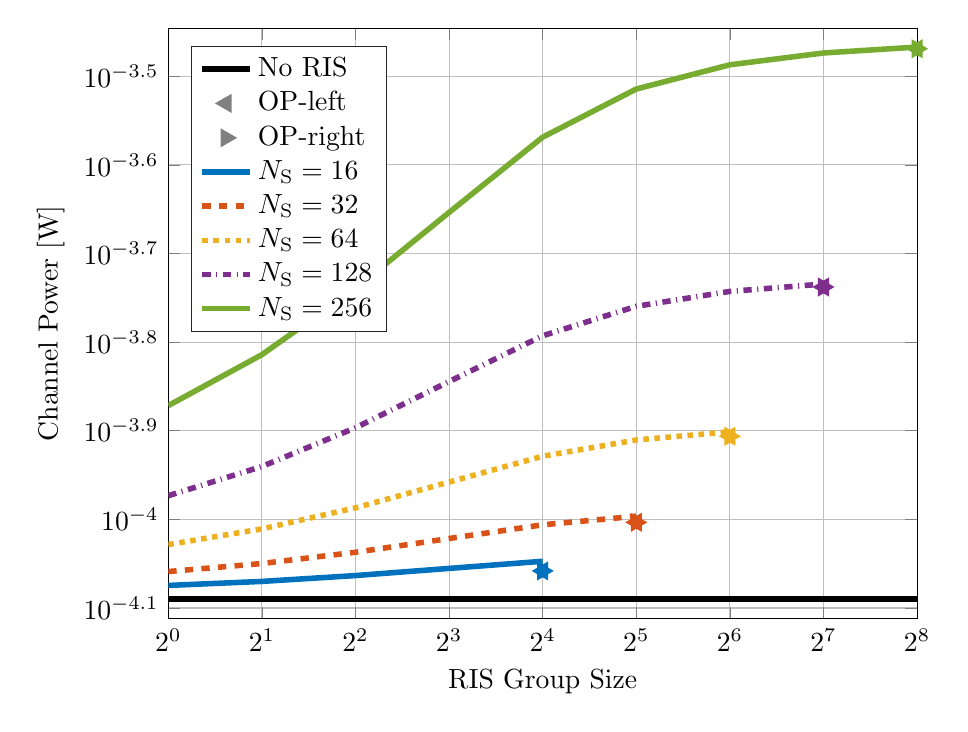
\begin{tikzpicture}

\begin{axis}[%
width=9.509cm,
height=7.5cm,
at={(0cm,0cm)},
scale only axis,
xmin=1,
xmax=9,
xtick={1,2,3,4,5,6,7,8,9},
xticklabels={{$2^0$},{$2^1$},{$2^2$},{$2^3$},{$2^4$},{$2^5$},{$2^6$},{$2^7$},{$2^8$}},
% xlabel style={font=\color{white!15!black}},
xlabel={RIS Group Size},
ymode=log,
ymin=7.71952537202106e-05,
ymax=0.000358145391898644,
yminorticks=true,
% ylabel style={font=\color{white!15!black}},
ylabel={Channel Power [W]},
axis background/.style={fill=white},
xmajorgrids,
ymajorgrids,
yminorgrids,
legend style={at={(0.03,0.97)}, anchor=north west, legend cell align=left, align=left, draw=white!15!black}
]
\addplot [color=black, line width=2.0pt]
  table[row sep=crcr]{%
1	8.12581618107481e-05\\
2	8.12581618107481e-05\\
3	8.12581618107481e-05\\
4	8.12581618107481e-05\\
5	8.12581618107481e-05\\
6	8.12581618107481e-05\\
7	8.12581618107481e-05\\
8	8.12581618107481e-05\\
9	8.12581618107481e-05\\
};
\addlegendentry{No RIS}

\addplot[only marks, mark=triangle, mark options={rotate=90}, mark size=2pt, line width=2pt, draw=mycolor2, forget plot] table[row sep=crcr]{%
x	y\\
5	8.74153313091917e-05\\
};
\addplot[only marks, mark=triangle, mark options={rotate=270}, mark size=2pt, line width=2pt, draw=mycolor2, forget plot] table[row sep=crcr]{%
x	y\\
5	8.74291033971713e-05\\
};
\addplot[only marks, mark=triangle, mark options={rotate=90}, mark size=2pt, line width=2pt, draw=mycolor5, forget plot] table[row sep=crcr]{%
x	y\\
6	9.91843205545709e-05\\
};
\addplot[only marks, mark=triangle, mark options={rotate=270}, mark size=2pt, line width=2pt, draw=mycolor5, forget plot] table[row sep=crcr]{%
x	y\\
6	9.91780210311253e-05\\
};
\addplot[only marks, mark=triangle, mark options={rotate=90}, mark size=2pt, line width=2pt, draw=mycolor8, forget plot] table[row sep=crcr]{%
x	y\\
7	0.00012405412223482\\
};
\addplot[only marks, mark=triangle, mark options={rotate=270}, mark size=2pt, line width=2pt, draw=mycolor8, forget plot] table[row sep=crcr]{%
x	y\\
7	0.000124044149009442\\
};
\addplot[only marks, mark=triangle, mark options={rotate=90}, mark size=2pt, line width=2pt, draw=mycolor11, forget plot] table[row sep=crcr]{%
x	y\\
8	0.000182844868229739\\
};
\addplot[only marks, mark=triangle, mark options={rotate=270}, mark size=2pt, line width=2pt, draw=mycolor11, forget plot] table[row sep=crcr]{%
x	y\\
8	0.000182852647982853\\
};
\addplot[only marks, mark=triangle, mark options={rotate=90}, mark size=2pt, line width=2pt, draw=mycolor12, forget plot] table[row sep=crcr]{%
x	y\\
9	0.000339584399340245\\
};
\addplot[only marks, mark=triangle, mark options={rotate=270}, mark size=2pt, line width=2pt, draw=mycolor12, forget plot] table[row sep=crcr]{%
x	y\\
9	0.000339587956470715\\
};


\addplot[draw=none, only marks, mark=triangle, mark options={rotate=90}, mark size=2pt, line width=2pt, draw=mycolor13] table[row sep=crcr]{%
x	y\\
1	1\\
};
\addlegendentry{OP-left}

\addplot[draw=none, only marks, mark=triangle, mark options={rotate=270}, mark size=2pt, line width=2pt, draw=mycolor13] table[row sep=crcr]{%
x	y\\
1	1\\
};
\addlegendentry{OP-right}

\addplot [color=mycolor2, line width=2.0pt]
  table[row sep=crcr]{%
1	8.41788427928869e-05\\
2	8.50641788557691e-05\\
3	8.63696852707132e-05\\
4	8.79903454326538e-05\\
5	8.96339735645668e-05\\
};
\addlegendentry{$N_\mathrm{S} = 16$}

\addplot [color=mycolor5, dashed, line width=2.0pt]
  table[row sep=crcr]{%
1	8.72783634122255e-05\\
2	8.91184079692796e-05\\
3	9.17640563659579e-05\\
4	9.50977289249081e-05\\
5	9.85503564245316e-05\\
6	0.00010076742152366\\
};
\addlegendentry{$N_\mathrm{S} = 32$}

\addplot [color=mycolor8, dotted, line width=2.0pt]
  table[row sep=crcr]{%
1	9.36120443845964e-05\\
2	9.75056089045287e-05\\
3	0.000102998044584118\\
4	0.000110120638452998\\
5	0.0001177772588008\\
6	0.000122854470762259\\
7	0.000125497666976946\\
};
\addlegendentry{$N_\mathrm{S} = 64$}

\addplot [color=mycolor11, dashdotted, line width=2.0pt]
  table[row sep=crcr]{%
1	0.000106289915229579\\
2	0.000114680256721358\\
3	0.000126826397397359\\
4	0.000142994695102657\\
5	0.00016107230730003\\
6	0.000173889895707073\\
7	0.000180752926606848\\
8	0.000184267352458571\\
};
\addlegendentry{$N_\mathrm{S} = 128$}

\addplot [color=mycolor12, line width=2.0pt]
  table[row sep=crcr]{%
1	0.000134334856638143\\
2	0.000153364621257308\\
3	0.000182125698990213\\
4	0.000221951821498391\\
5	0.000269865717893532\\
6	0.000305861046930524\\
7	0.00032571637890533\\
8	0.000335868097136638\\
9	0.00034109084942728\\
};
\addlegendentry{$N_\mathrm{S} = 256$}

\end{axis}

\end{tikzpicture}%
